\documentclass[16pt, a4paper, two column]{article}
\usepackage[utf8]{inputenc}
\usepackage{mathtools}
\usepackage[a4paper, total={6in, 8in}, margin = 1in]{geometry}
\usepackage{enumitem}
\usepackage{graphicx}
\graphicspath{{images/}}
\usepackage{amsmath}
\newcommand{\myvec}[1]{\ensuremath{\begin{pmatrix}#1\end{pmatrix}}}
\let\vec\mathbf
\title{AI1110 Assignment 1}
\author{Abhishek Kumar, AI21BTECH11003}
\begin{document}
\maketitle
\section*{Question 1a}
Solve the following inequation, write down the solution set and represent it on the real number line:
\begin{align*}
  11x-4 < 15x + 4 \le 14 + 13x,  x\in \mathbb{W} 
\end{align*}
\section*{Solution}
\begin{align}
  -4 + 11x < 15x + 4 \le 14 + 13x,  x\in \mathbb{W} 
\end{align}


now consider each equation in this expression as a line,i.e., $L_1$ $L_2$ ans $L_3$
\begin{align}
L_1 &\equiv 11x-y-4  \\
L_2 &\equiv 15x-y+4 \\
L_3 &\equiv 13x-y+14
\end{align}

In vector form,
\begin{align}
	L_1 &\equiv \myvec{11 & -1}\vec{x} = 4 \\
	L_2 &\equiv \myvec{15 & -1} \vec{x} = -4 \\
	L_3 &\equiv \myvec{13 & -1}\vec{x} = -14
\end{align}
So we need to find the range of x at where the line $L_2$ lies between between line $L_1$ and the line $L_3$

We can obtain the intersection point of $L_1$ and $L_2$ by the following way,
\begin{align}
	\myvec{11 & -1 \\
		15 & -1}\vec{x} &= \myvec{4 \\ -4} 
\end{align}
The augmented matrix for the above matrix equation is 
\begin{align}
	\myvec{ 11 & -1 & \vrule & 4 \\
		15 & -1 & \vrule & -4} \\
	\xleftrightarrow[]{R_1 \leftarrow R_1-R_2}
		\myvec{ -4 & 0 & \vrule & 8 \\
			15 & -1 & \vrule & -4} \\
	\xleftrightarrow[]{R_1 \leftarrow R_1/-4}
		\myvec{ 1 & 0 & \vrule & -2 \\
			15 & -1 &\vrule & -4} \\
	\xleftrightarrow[]{R_2 \leftarrow R_2-15R_1}
		\myvec{ 1 & 0 & \vrule & -4 \\
			0 & -1 & \vrule & 26} \\
	\xleftrightarrow[]{ R_2 \leftarrow R_2/-1}
		\myvec{ 1 & 0 & \vrule & -4 \\
			0 & 1 & \vrule & -26} \\
	\implies \vec{x} = \myvec{-4 \\ -26}
\end{align}
Hence the point of intersection of lines $L_1$ and $L_2$ is $\myvec{-4 \\ -26}$ .\newline
Similarly we get the x value at intersection point of lines $L_2$ and $L_3$
\begin{align}
	\myvec{15 & -1 \\
		13 & -1}\vec{x} &= \myvec{-4 \\ -14}
\end{align}
The augmented matrix for the above matrix equation is 
\begin{align}
	\myvec{ 15 & -1 & \vrule & -4 \\
		13 & -1 & \vrule & -14} \\
	\xleftrightarrow[]{R_1 \leftarrow R_1-R_2}
		\myvec{ 2 & 0 & \vrule & 10 \\
			13 & -1 & \vrule & -14} \\
	\xleftrightarrow[]{R_1 \leftarrow R_1/2}
		\myvec{ 1 & 0 & \vrule & 5 \\
			13 & -1 &\vrule & -14} \\
	\xleftrightarrow[]{R_2 \leftarrow R_2-13R_1}
		\myvec{ 1 & 0 & \vrule &  4.67\\
			0 & -1 & \vrule & -79} \\
	\xleftrightarrow[]{R_2 \leftarrow R_2/-1}
		\myvec{ 1 & 0 & \vrule &  5\\
			0 & 1 & \vrule & 79} \\
	\implies \vec{x} = \myvec{5 \\ 79}
\end{align}
Hence the point of intersection of lines $L_2$ and $L_3$ is $\myvec{5 \\ 79}$.\newline
%\vspace{16pt}

Since $L_1 < L_2 \le L_3$, this implies the corresponding x-coordinates follows, $-2< x \le 5$  and x\in \mathbb{W}\newline


\begin{figure}[h]
  %  \centering
    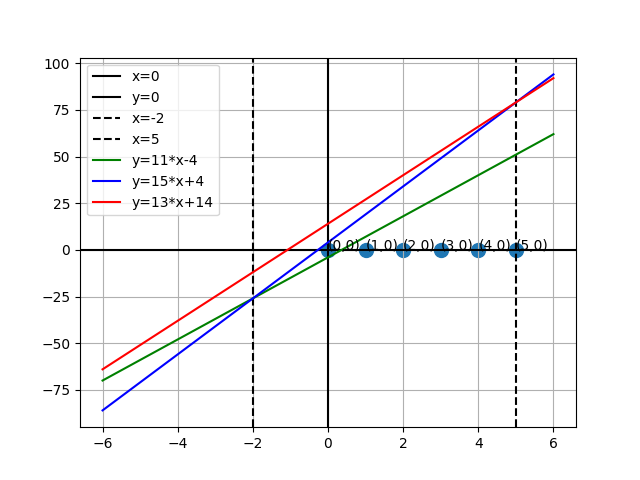
\includegraphics[width=\columnwidth]{Figure_3}
    \caption{lines $L_1$, $L_2$ and $L_3$}
    
\end{figure}

%\vspace{16pt}





%\vspace{10pt}
\noindent Therefore the whole numbers in this range are,

\begin{center}
\begin{tabular}{|c|}
\hline
\textbf{$ \{  0, 1, 2, 3, 4,5\}$} \\
\hline
\end{tabular}
\end{center}


\noindent Here is the plot of corresponding points on the real number line\\
\begin{figure}[h]
   % \centering
    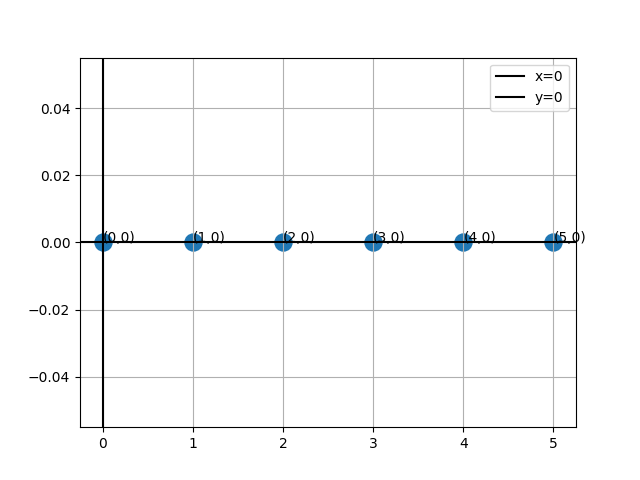
\includegraphics[width =\columnwidth]{Figure_4}
    \caption{set of points that obey given expression on real number line}
    \label{fig:mesh1}
\end{figure}
\end{document}